\documentclass[]{beamer}
\usetheme{Dresden}
% \useoutertheme{split}

\usepackage{color}
\usepackage{graphicx}
\usepackage{listings}
\usepackage{lmodern} %% allow bold keywords
\usepackage{menukeys}
\usepackage{qtree}

\definecolor{darkgreen}{rgb}{0,0.5,0}
\definecolor{lightblue}{rgb}{0.2,0.2,1}

\lstset{language=Java,
	basicstyle=\ttfamily\footnotesize,
	keywordstyle=\color{purple},
	commentstyle=\color{darkgreen},
	numberstyle=\tiny\color{gray},
	stringstyle=\color{blue},
	tabsize=4,
	showstringspaces=false,
	breaklines=true,
	keepspaces=true,
	numbers=left,
	escapechar=@
}

\title{Java}
\subtitle{Generics and Collections}
\author{Nico Westerbeck}
\date{\today}

\begin{document}

\begin{frame}
\titlepage
\end{frame}
\begin{frame}{Overview}
\tableofcontents
\end{frame}

\section{Introduction}

\subsection{Last session}
\begin{frame}{Inheritance}
	\begin{center}
		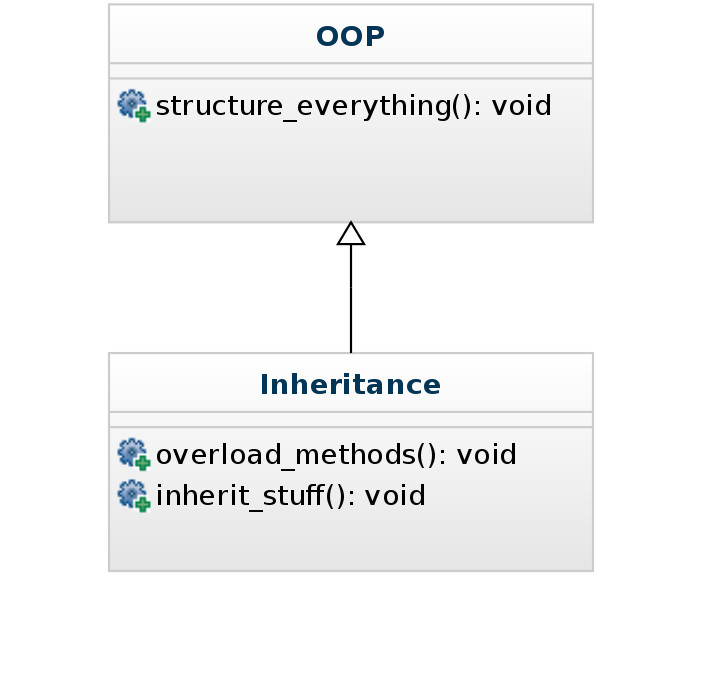
\includegraphics[height=7cm]{res/inheritance-diagram.jpg}
	\end{center}
\end{frame}

\section{Static Methods}
\subsection{Static Methods}
\begin{frame}[fragile]{Calling static Methods}
\begin{lstlisting}
	class EnrollmentSystem {
		public static void doSomething() {
		}
	}
	
	[...]
	EnrollmentSystem example = new EnrollmentSystem();
	example.doSomething(); // Works
	
	EnrollmentSystem.doSomething();  // Works aswell
	
\end{lstlisting}
\end{frame}

\begin{frame}[fragile]{No fields available!}
\begin{lstlisting}
	class EnrollmentSystem {
		private int x;
		
		public static void doSomething() {
			x = 5;  // Does not work!
		}
	}
\end{lstlisting}
\end{frame}

\begin{frame}[fragile]{No fields available!}
\begin{lstlisting}
	class EnrollmentSystem {
		private static int x;
		
		public static void doSomething() {
			x = 5;  // Works
		}
	}
\end{lstlisting}
Avoid this unless you know what it does!
\end{frame}

\section{A glimpse into Generics}
\subsection{What is a generic}
\begin{frame}[fragile]{Generics}
	% Ask who has seen something like this already
	\begin{lstlisting}
	List<Tutor> list1 = new LinkedList<Tutor>();
	List<Student> list2 = new LinkedList<Student>();
	\end{lstlisting}

\end{frame}

\begin{frame}[fragile]{Generics}
% Bad example, but okay for first impression
% Bad because: 
%  An array is not linked
%  A fixed array size is evil
%  An array is somewhat tricky to initialise generically
\begin{lstlisting}
public class LinkedList<T> {
	T[] items;
	int nextFreeItem;
	
	public void add(T newItem) {
		items[nextFreeItem] = newItem;
		nextFreeItem++;
	}
}
\end{lstlisting}
\end{frame}

\begin{frame}{Why they suck}
	\begin{itemize}
		\item You can not use operators on them
		\item Compile-time-generics only
		\item Can't use builtin-types, needs wrapper classes (see next slides)
		\item Wildcarting: List<?>
	\end{itemize}
	$=>$ I won't teach them in detail
\end{frame}

\subsection{Wrapper Classes}

\begin{frame}[fragile]{Wrapper Class}
	Primitive data types can not be elements in collections. 
	Use wrapper classes like \emph{Integer} instead.
	\begin{lstlisting}[basicstyle=\ttfamily\scriptsize]
	public static void main(String[] args) {
	
	    LinkedList<Integer> list = new LinkedList<Integer>();
	    
	    list.add(3); 
	    list.addFirst(1);
	    list.add(3);
	    list.add(8);
	    list.remove(3); // remove the 4th element
	    list.add(7);
	    
	    System.out.println(list); // prints: [1, 3, 3, 7]
	}
	\end{lstlisting}
\end{frame}

\begin{frame}{Wrapper Class}
	\begin{center}
		\begin{tabular}{ c  c }
			boolean & Boolean \\
			byte & Byte \\
			char & Character \\
			int & Integer \\
			float & Float \\
			double & Double \\
			long & Long \\
			short & Short
		\end{tabular}
	\end{center}
\end{frame}

\begin{frame}[fragile]{Wrapper Class}
	Wrapper classes hold extra functionality related to their datatype
	\begin{lstlisting}[basicstyle=\ttfamily\scriptsize]
	public static void main(String[] args) {
	
	    Integer example = Integer.valueOf("12345");
	    
	    System.out.println(example);  // Prints 12345
	    
	    System.out.println(Integer.toBinaryString(example)); // Prints 11000000111001
	    
	}
	\end{lstlisting}
\end{frame}

\section{Collections}
\subsection{Overview}
\begin{frame}{Collections Framework}
	Java offers various data structures like \textbf{Sets}, \textbf{Lists} and \textbf{Maps}.
	Those structures are part of the collections framework.
	\vfill
	There are interfaces to access the data structures in an easy way.
	There are multiple implementations for various needs.
	Alternatively you can use your own implementations.
	\vfill
	For more information visit:
	\begin{itemize}
		\item \scriptsize\url{https://docs.oracle.com/javase/7/docs/api/java/util/Collection.html}
		\item \url{https://docs.oracle.com/javase/7/docs/api/java/util/Set.html}
		\item \url{https://docs.oracle.com/javase/7/docs/api/java/util/List.html}
		\item \url{https://docs.oracle.com/javase/7/docs/api/java/util/Map.html}
	\end{itemize}
\end{frame}

\subsection{Set and List}
\begin{frame}[fragile]{Set}
	A set is a collection that holds one type of objects.
	A set can not contain one element twice.
	Like all collections the interface \emph{Set} is part of the package \texttt{java.util}.
	\begin{lstlisting}[basicstyle=\ttfamily\scriptsize]
	import java.util.*;

	public class TestSet {
	    
	    public static void main(String[] args) {
	        Set<String> set = new HashSet<String>();
	    
	        set.add("foo");
	        set.add("bar");
	        set.remove("foo");
	        System.out.println(set); // prints: [bar]
	    }
	}
	\end{lstlisting}
	In the following examples \texttt{import java.util.*;} will be omitted.
\end{frame}

\begin{frame}[fragile]{List}
	A list is an ordered collection.
	\vfill
	The implementation \texttt{LinkedList} is a double-linked list.
	\begin{lstlisting}[basicstyle=\ttfamily\scriptsize]
	public static void main(String[] args) {
	
	    List<String> list = new LinkedList<String>();
	    
	    list.add("foo"); 
	    list.add("foo"); // insert "foo" at the end
	    list.add("bar");
	    list.add("foo");
	    list.remove("foo"); // removes the first "foo"
	    
	    System.out.println(list); // prints: [foo, bar, foo]
	}
	\end{lstlisting}
\end{frame}
	
\begin{frame}[fragile]{List Methods}
	some useful List methods:\\
	\vspace{1em}
	\begin{tabular}{ r l r }
		void & \texttt{add(int index, E element)}
		& \footnotesize{insert element at position index} \\
		E &\texttt{get(int index)}
		& \footnotesize{get element at position index} \\
		E &\texttt{set(int index, E element)}
		& \footnotesize{replace element at position index} \\
		E &\texttt{remove(int index)}
		& \footnotesize{remove element at position index}
	\end{tabular}
	\vfill
	some useful LinkedList methods:\\
	\vspace{1em}
	\begin{tabular}{ r l r }
		void & \texttt{addFirst(E element)}
		& \footnotesize{append element to the beginning} \\
		E & \texttt{getFirst()}
		& \footnotesize{get first element} \\
		void & \texttt{addLast(E element)}
		& \footnotesize{append element to the end} \\
		E & \texttt{getLast()}
		& \footnotesize{get last element}
	\end{tabular}
\end{frame}

\subsection{Iterating}
\begin{frame}[fragile]{For Loop}
	The for loop can iterate over every element of a collection:\\
	\hspace{1em}\texttt{for (E e : collection)}
	\begin{lstlisting}
	public static void main(String[] args) {
	
	    List<Integer> list = 
	        new LinkedList<Integer>();
	    
	    list.add(1);
	    list.add(3);
	    list.add(3);
	    list.add(7);
	    
	    for (Integer i : list) {
	        System.out.print(i + " "); // prints: 1 3 3 7
	    }
	}
	\end{lstlisting}
\end{frame}

\begin{frame}[fragile]{Iterator}
	An iterator iterates step by step over a collection.
	\begin{lstlisting}[basicstyle=\ttfamily\scriptsize]
	public static void main(String[] args) {
	
	    List<Integer> list = new LinkedList<Integer>();
	    
	    list.add(1);
	    list.add(3);
	    list.add(3);
	    list.add(7);
	    
	    Iterator<Integer> iter = list.iterator();
	    
	    while (iter.hasNext()) {
	        System.out.print(iter.next());
	    }
	    // prints: 1337
	}
	\end{lstlisting}
\end{frame}

\begin{frame}[fragile]{Iterator}
	A standard iterator has only three methods:
	\begin{itemize}
	\item \texttt{boolean hasNext()} - indicates if therer are more elements
	\item \texttt{E next()} - returns the next element
	\item \texttt{void remove()} - returns the current element
	\end{itemize}
	\vspace{1em}
	The iterator is instanced via \texttt{collection.iterator()} :
	\begin{lstlisting}[basicstyle=\ttfamily\scriptsize]
	    Collection<E> collection = new Implementation<E>;
	    Iterator<E> iter = collection.iterator();
	\end{lstlisting}
	Special iterators like \emph{ListIterator} are more sophisticated.
\end{frame}

\subsection{Map}
\begin{frame}[fragile]{Map}
	The interface \emph{Map} is not a subinterface of \emph{Collection}.\\
	A map contains pairs of key and value. Each key refers to a value. 
	Two keys can refer to the same value. There are not two equal keys in one map.
	\emph{Map} is part of the package \texttt{java.util}.
	\vfill
	\begin{lstlisting}[basicstyle=\ttfamily\scriptsize]
	public static void main (String[] args) {
	
	    Map<Integer, String> map = 
	        new HashMap<Integer, String>();
	    
	    map.put(23, "foo");
	    map.put(28, "foo");
	    map.put(31, "bar");
	    map.put(23, "bar"); // "bar" replaces "foo" for key = 23
	    
	    System.out.println(map);
	    // prints: {23=bar, 28=foo, 31=bar}
	}
	\end{lstlisting}
\end{frame}

\begin{frame}[fragile]{KeySet and Values}
	You can get the set of keys from the map.
	Because one value can exist multiple times a collection is used for the values.
	\begin{lstlisting}[basicstyle=\ttfamily\scriptsize]
	public static void main (String[] args) {
	
	    // [...] map like previous slide
	    
	    Set<Integer> keys = map.keySet();
	    Collection<String> values = map.values();
	    
	    System.out.println(keys);
	    // prints: [23, 28, 31]
	    
	    System.out.println(values);
	    // prints: [bar, foo, bar]
	}
	\end{lstlisting}
\end{frame}

\begin{frame}[fragile]{Iterator}
	Therer is no iterator for maps. 
	To iterate over a map use the iterator from the set of keys.
	\begin{lstlisting}[basicstyle=\ttfamily\scriptsize]
	public static void main (String[] args) {
	
	    // [...] map, keys, values like previous slide    	    
	    Iterator<Integer> iter = keys.iterator();
	    
	    while(iter.hasNext()) {
	        System.out.print(map.get(iter.next()) + " ");
	    } // prints: bar foo bar
	    
	    System.out.println(); // print a line break
	    
	    for(Integer i: keys) {
	        System.out.print(map.get(i) + " ");
	    } // prints: bar foo bar
	}
	\end{lstlisting}
\end{frame}

\begin{frame}[fragile]{Nested Maps}
	Nested maps offer storage with key pairs.
	\begin{lstlisting}[basicstyle=\ttfamily\scriptsize]
	public static void main (String[] args) {		
	
	    Map<String, Map<Integer, String>> addresses = 
		    new HashMap<String, Map<Integer, String>>();
		
	    addresses.put("Noethnitzer Str.", 
	        new HashMap<Integer, String>());
		
	    addresses.get("Noethnitzer Str.").
	        put(46, "Andreas-Pfitzmann-Bau");
	    addresses.get("Noethnitzer Str.").
	        put(44, "Fraunhofer IWU");
	}
	\end{lstlisting}
\end{frame}

\begin{frame}{Overview}
	\begin{center}
		\begin{tabular}{ l | l }
			List & Keeps order of objects \\
				 & Easily traversible \\
				 & Search not effective \\
			\hline
			Set  & No duplicates \\
				 & No order - still traversible \\
				 & Effective searching \\
			\hline
			Map  & Key-Value storage \\
				 & "Search" super-effective \\
				 & Traversing difficult
			
		\end{tabular}
	\end{center}
\end{frame}

\end{document}